\documentclass[
  11pt,
  letterpaper,
   addpoints,
   answers
  ]{exam}

\usepackage{../exercise-preamble}

\begin{document}

\noindent
\begin{minipage}{0.47\textwidth}

\includegraphics[width=\textwidth]{../fcfm_die}
\end{minipage}
\begin{minipage}{0.53\textwidth}
\begin{center} 
\large\textbf{Análisis de Sistemas Dinámicos y Estimación} (EL3204-2) \\
\large\textbf{Clase auxiliar 1} \\
\normalsize Prof.~Heraldo Rozas.\\
\normalsize Prof.~Aux.~Erik Saez - Maximiliano Morales
\end{center}
\end{minipage}

\vspace{0.5cm}
\noindent
\vspace{.85cm}

\begin{questions}
    %%%%%%%%%%%%%%%%%%%%%%%%%%%
    \question Considere el sistema de la siguiente figura, donde se tiene un carro atado a un resorte con un sensor de distancia, capaz de medir la distancia del carro a la pared. Suponga que existe una fuerza de fricción viscosa con la superficie $F_f$ de la forma $F_f = b_1 \dot{z} + b_2 \dot{z}^2$.
    \begin{figure}[h!]
        \centering
        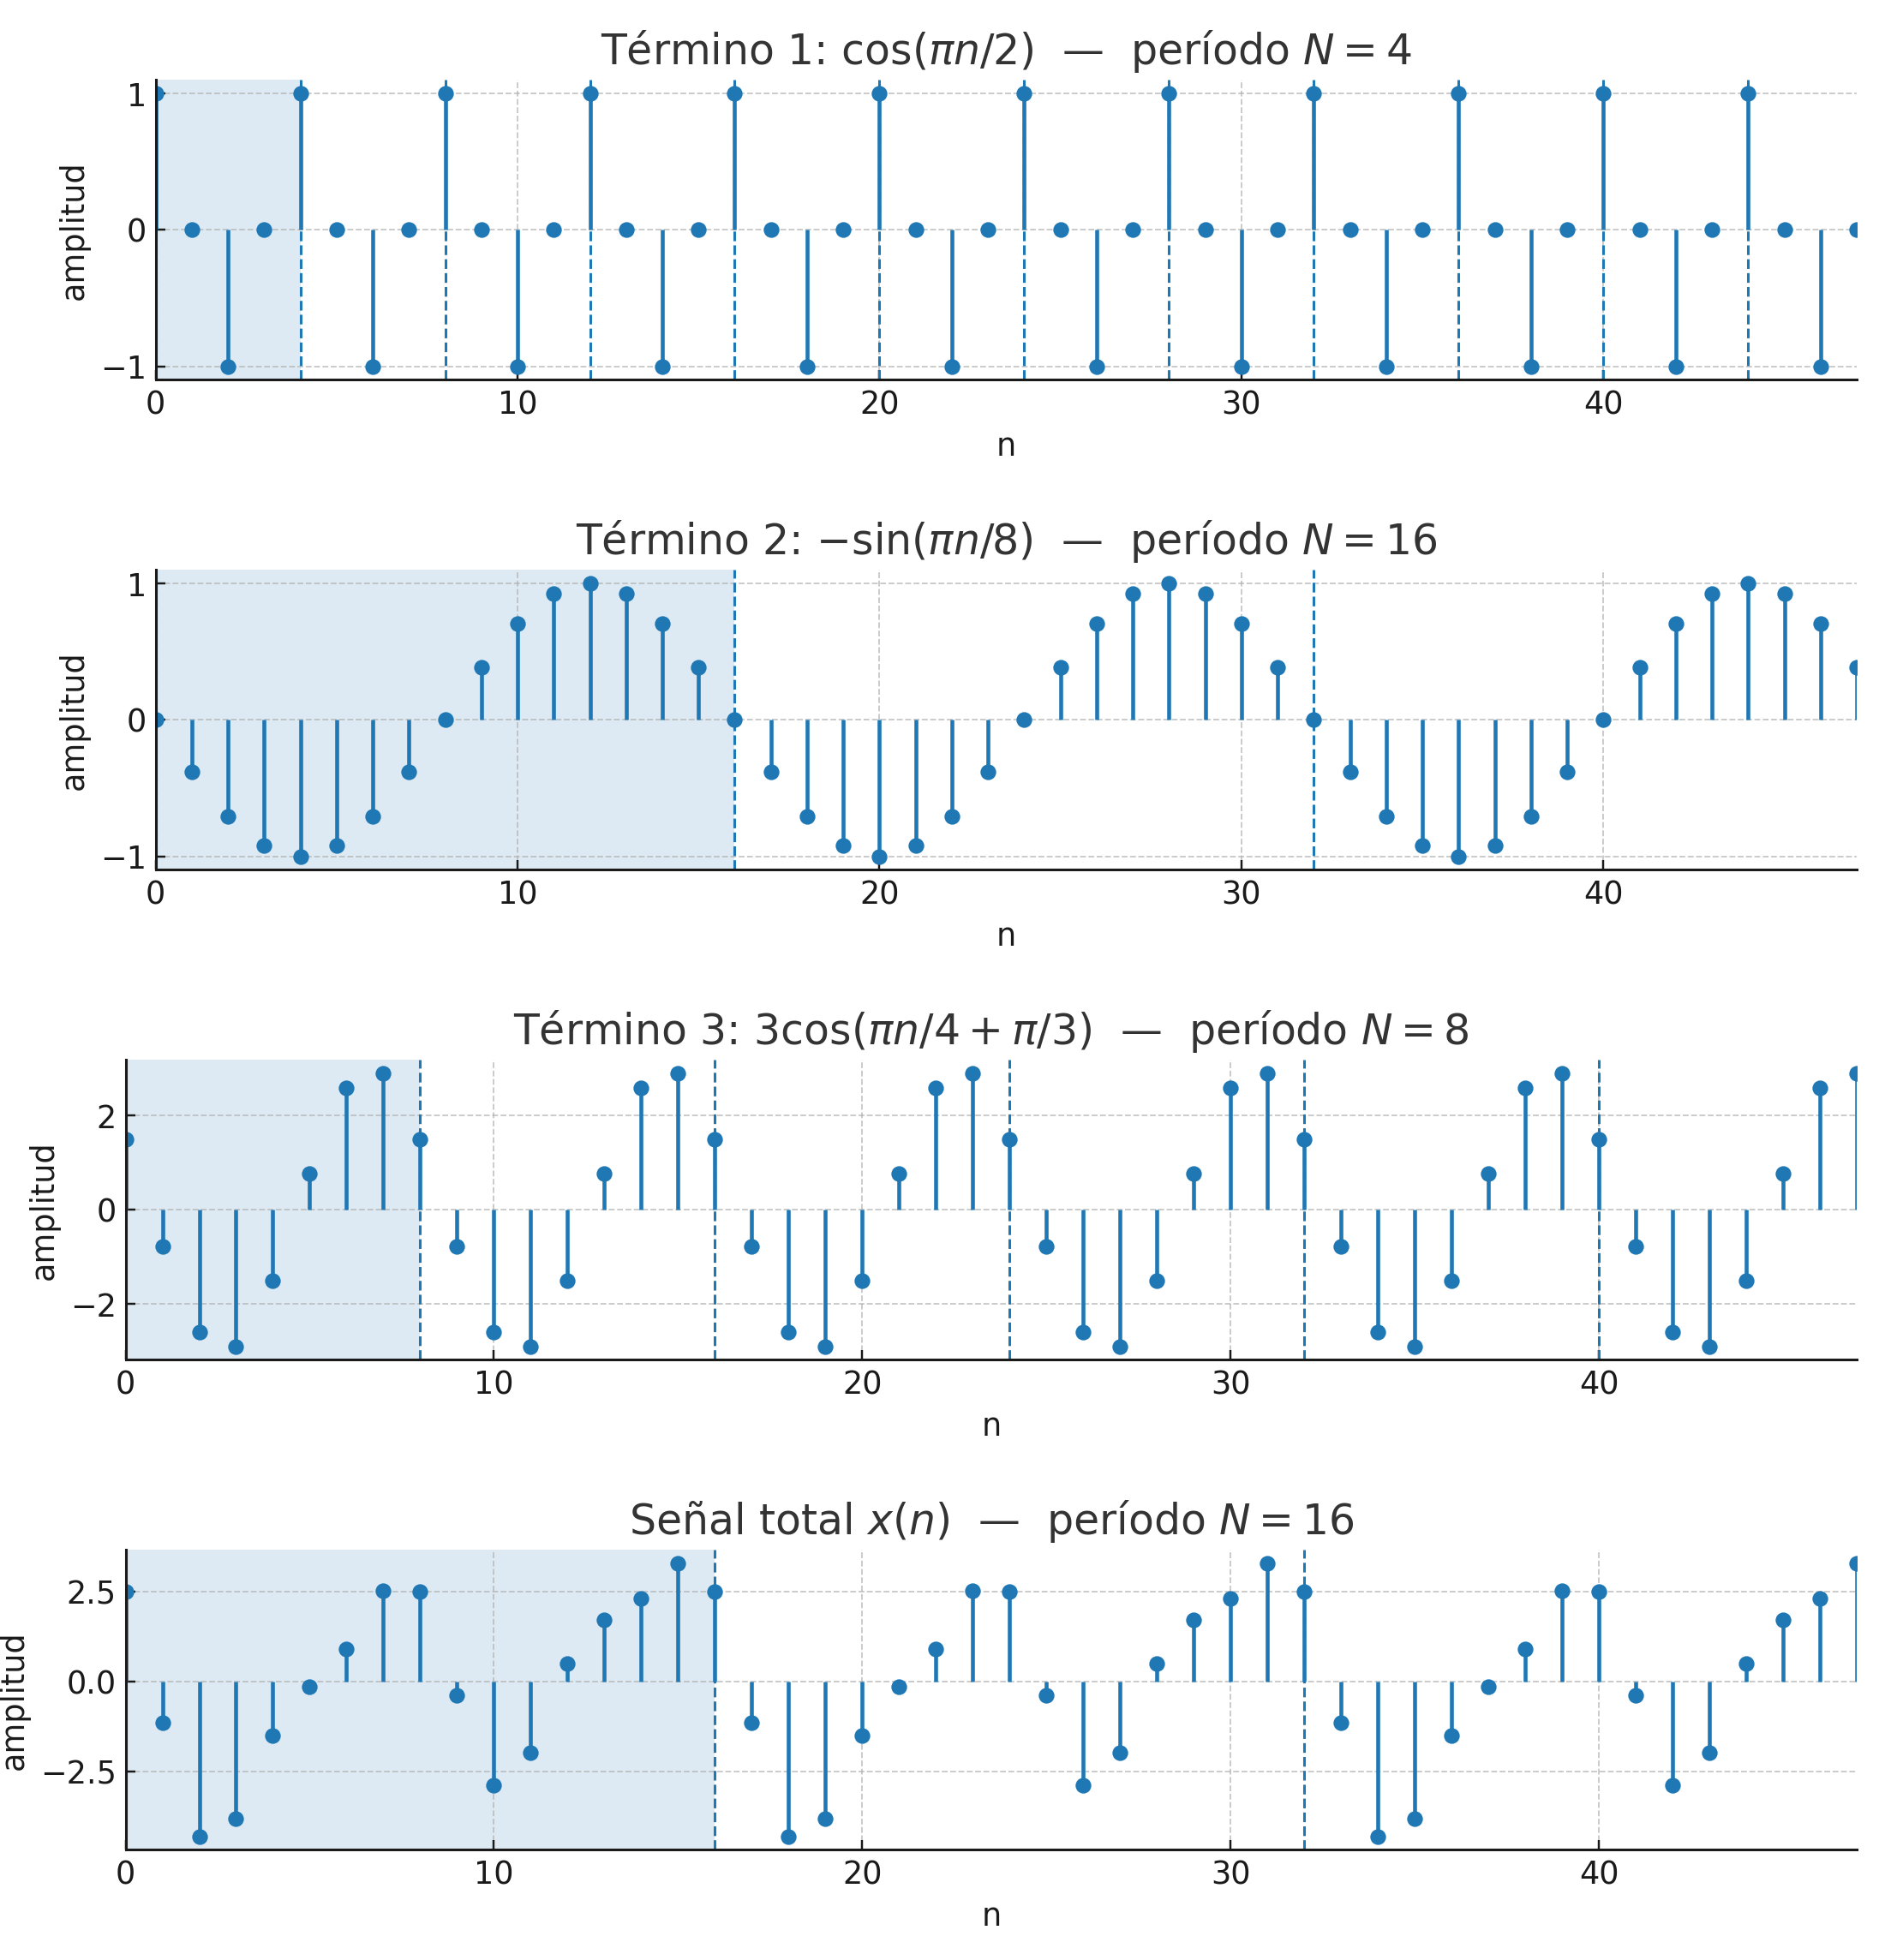
\includegraphics[width=0.5\textwidth]{Auxiliar_1_1}
    \end{figure}
    \begin{enumerate}
        \item Establezca hipótesis simplificatorias para el problema.
        \item Formule un modelo matemático del sistema que sea consistente con sus hipótesis.
        \item Encuentre el punto de operación que asegure $z = 1$ m.
    \end{enumerate}
    %%%%%%%%%%%%%%%%%%%%%%%%%%%
    \begin{solution}
        Para poder plantear un buen modelo, es necesario establecer hipótesis que simplifiquen el problema y lo hagan abordable. Estas hipótesis son muy importantes, ya que pueden complejizar o simplificar el problema cuanto sea necesario. 

Para este caso particular, algunas hipótesis que se pueden plantear para simplificar el problema son:

\begin{enumerate}
    \item El carro solamente se mueve horizontalmente.
    \item El resorte actúa en el régimen lineal, de acuerdo a la ley de Hooke.
    \item La constante elástica $k$ del resorte no varía, y su largo natural $l_0$ es 0.
    \item El roce es de la forma 
    \begin{equation}
        F_f = b_1 \dot{z} + b_2 \dot{z}^2.
    \end{equation}
    \item La fuerza $F(t)$ es conocida y varía en el tiempo.
\end{enumerate}

\section*{Modelo matemático}

Plantear un modelo matemático para un sistema físico se reduce, generalmente, a encontrar una ecuación diferencial que modela la dinámica del sistema. Para este caso particular, podemos utilizar segunda ley de Newton para obtener dicha ecuación diferencial.

Haciendo esto, por segunda ley de Newton tenemos
\begin{equation}
    m\ddot{z} = F(t) - F_e - F_f, \tag{2}
\end{equation}
donde $F_e$ corresponde a la fuerza elástica del resorte, y $F_f$ es la fuerza de roce. La fuerza elástica, por la segunda hipótesis, está dada por
\begin{equation}
    F_e = kz, \tag{3}
\end{equation}
por lo que la ecuación 2 es
\begin{equation}
    m\ddot{z} = F(t) - kz - b_1\dot{z} - b_2\dot{z}^2. \tag{4}
\end{equation}

Despejando $\ddot{z}$, tenemos que el modelo matemático es
\begin{equation}
    \ddot{z} = \frac{1}{m}F(t) - \frac{k}{m}z - \frac{b_1}{m}\dot{z} - \frac{b_2}{m}\dot{z}^2. \tag{5}
\end{equation}

\section*{Punto de operación}

Para encontrar el punto de operación, el objetivo es determinar el valor de la entrada $F(t)$ de modo tal que se tenga $z = 1 \, \text{m}$. Implícitamente, al hablar de punto de operación se requiere estaticidad (a menos que se indique lo contrario), por lo que podemos asumir que $z$ no varía, indicando que $\dot{z} = \ddot{z} = 0$.

Podemos utilizar lo anteriormente mencionado sobre el modelo, imponiendo las condiciones indicadas y encontrando el valor de $F(t)$ que las satisfaga. Imponiendo $z = 1$, $\dot{z} = \ddot{z} = 0$ sobre la ecuación 5 tenemos
\begin{equation}
    0 = \frac{1}{m}F(t) - \frac{k}{m} \quad \Rightarrow \quad F(t) = k,
\end{equation}
por lo que el punto de operación es $F(t) = k$. Un aspecto importante a notar es que, para encontrar este punto de operación, asumimos que la fuerza $F(t)$ es constante en el tiempo. Más adelante dentro del ramo (y en otros ramos de la carrera) veremos que considerar una fuerza constante no siempre es lo ideal, sino que es posible diseñar una entrada particular para llegar a la condición de estaticidad más rápidamente.

    \end{solution}
    %%%%%%%%%%%%%%%%%%%%%%%%%%%
    \question Considere el siguiente péndulo apoyado en un carro móvil, el cual se desliza por una barra.
    \begin{figure}[h!]
        \centering
        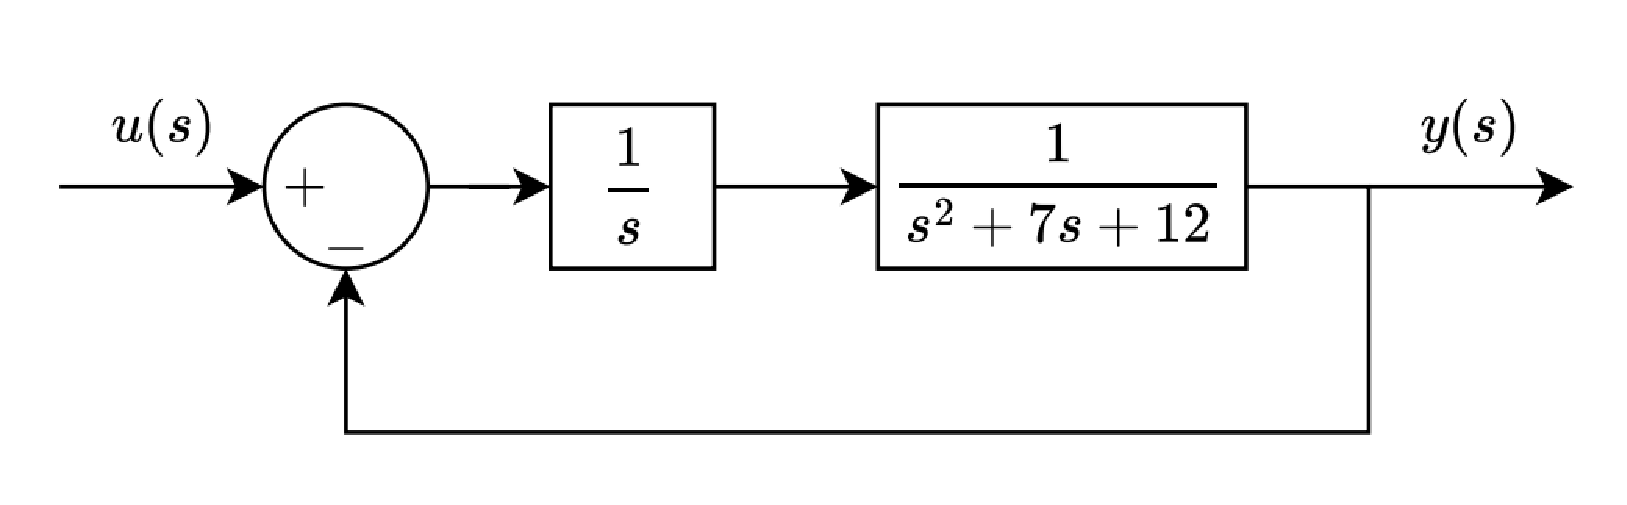
\includegraphics[width=0.5\textwidth]{Auxiliar_1_2}
    \end{figure}
    \begin{enumerate}
        \item Establezca hipótesis simplificatorias.
        \item Formule un modelo matemático, que capture la dinámica del sistema.
        \item Identifique entradas, salidas y estados en su modelo.
        \item Linealice en torno a $\theta = \pi$.
    \end{enumerate}
%%%%%%%%%%%%%%%%%%%%%%%%%%%
\begin{solution}
    Al igual que en el ejercicio anterior, es necesario establecer buenas hipótesis simplificatorias para que el problema sea abordable. Algunas de estas hipótesis que podemos plantear son las siguientes:

\begin{enumerate}
    \item El carro tiene masa negligible.
    \item La vara del péndulo no tiene masa.
    \item La vara del péndulo es rígida.
    \item La bola del péndulo es una masa puntual.
    \item No hay roce con el aire.
    \item Solamente existe movimiento en los dos ejes ilustrados.
\end{enumerate}

\subsection{Modelo matemático}

Utilizando las hipótesis planteadas, podemos encontrar un modelo matemático. Para esto, si bien se podría utilizar la segunda ley de Newton para plantear una ecuación diferencial, al ser un péndulo este es un proceso engorroso: en cambio, utilizaremos mecánica Lagrangiana para plantear la ecuación diferencial.

El objetivo de esto es utilizar el Lagrangiano $L = T - V$, con $T$ la energía cinética y $V$ la energía potencial, junto a la ecuación de Euler-Lagrange
\begin{equation}
    \frac{\partial L}{\partial q_j} - \frac{d}{dt} \left( \frac{\partial L}{\partial \dot{q}_j} \right) = 0, \tag{7}
\end{equation}
y, a partir de esta ecuación, obtener la edo. También, es importante notar que la ecuación de Euler-Lagrange planteada de esa manera es válida si no existen pérdidas de energía en el sistema: si hubiesen fuerzas no conservativas, se deberían considerar dentro de la ecuación. Este supuesto es válido debido a la hipótesis de que no hay roce.

Para calcular el Lagrangiano, debemos comenzar calculando la energía cinética. Dado que solamente la bola del péndulo tiene masa, este será el único componente con energía cinética. Si llamamos $x_p, y_p$ a la posición del péndulo, podemos notar que esta se puede escribir como
\begin{equation}
    x_p = x + l \sin \theta \quad y_p = -l \cos \theta,
\end{equation}
donde asumimos que $y$ es positivo hacia arriba, que $y = 0$ corresponde a la ubicación de la barra, y que se tiene una distancia $x(t)$ desde el origen a la vertical del péndulo. Con estas posiciones, la energía cinética estará dada por
\begin{equation}
    T = \frac{1}{2} m \left( \dot{x}_p^2 + \dot{y}_p^2 \right). \tag{9}
\end{equation}

Calculando las derivadas, tenemos
\begin{equation}
    \dot{x}_p = \dot{x} + l \dot{\theta} \cos \theta \quad \dot{y}_p = l \dot{\theta} \sin \theta, \tag{10}
\end{equation}
donde los términos $\dot{\theta}$ salen por regla de la cadena. Utilizándolos para calcular la energía cinética, tenemos
\begin{equation}
    T = \frac{1}{2} m \left( \dot{x}^2 + \dot{x} l \dot{\theta} \cos \theta + l^2 \dot{\theta}^2 \cos^2 \theta + l^2 \dot{\theta}^2 \sin^2 \theta \right). \tag{11}
\end{equation}

Podemos notar que
\begin{equation}
    l^2 \dot{\theta}^2 \cos^2 \theta + l^2 \dot{\theta}^2 \sin^2 \theta = l^2 \dot{\theta}^2 (\cos^2 \theta + \sin^2 \theta) = l^2 \dot{\theta}^2, \tag{12}
\end{equation}
por lo que
\begin{equation}
    T = \frac{1}{2} m \left( \dot{x}^2 + 2 \dot{x} l \dot{\theta} \cos \theta + l^2 \dot{\theta}^2 \right) = \frac{1}{2} m \dot{x}^2 + m l \dot{x} \dot{\theta} \cos \theta + \frac{1}{2} m l^2 \dot{\theta}^2. \tag{13}
\end{equation}

Para la energía potencial, dado que el único componente que tiene masa es la bola del péndulo, solamente se tiene la contribución de su energía potencial gravitatoria. Además, dado que la vara es rígida, sabemos que no actúa como un resorte, y, por ende, no hay energía potencial elástica. Considerando todo esto, la energía potencial $V$ está dada por
\begin{equation}
    V = mgy_p = -mgl \cos \theta. \tag{14}
\end{equation}

Luego, el Lagrangiano es
\begin{equation}
    L = \frac{1}{2} m \left( \dot{x}^2 + 2 \dot{x} l \dot{\theta} \cos \theta + l^2 \dot{\theta}^2 \right) + mgl \cos \theta. \tag{15}
\end{equation}

Para poder considerar el Lagrangiano dentro de la ecuación de Euler-Lagrange, es necesario calcular las derivadas de cada término. Dado que estamos trabajando en coordenadas polares, sabemos que hay dos coordenadas: el radio \(r\) y el ángulo \(\theta\). Dado que \(r = l\) es constante, sabemos que no hay dinámica en la dirección radial, por lo que solamente nos interesa analizar la dinámica angular. Esto significa que debemos calcular las derivadas de \(L\) con respecto a \(\theta\) y \(\dot{\theta}\).
Calculando las derivadas, tenemos
\begin{equation}
    \frac{\partial L}{\partial \theta} = -mgl \sin \theta - ml \dot{x} \sin \theta \tag{20}
\end{equation}
\begin{equation}
    \frac{\partial L}{\partial \dot{\theta}} = ml^2 \dot{\theta} + ml \dot{x} \cos \theta. \tag{21}
\end{equation}

Un punto importante notar a la hora de calcular las derivadas, es que, al derivar con respecto a \(\theta\), se debe tener en cuenta que \(\dot{\theta}\) no depende de \(\theta\), sino que solamente del tiempo. Lo mismo aplica a la hora de derivar con respecto a \(\dot{\theta}\), en donde \(\dot{\theta}\) actúa como una constante.
Luego, usando la ecuación 21 podemos tomar la derivada con respecto al tiempo, de lo que tenemos
\begin{equation}
    \frac{d}{dt} \left( \frac{\partial L}{\partial \dot{\theta}} \right) = \frac{d}{dt} \left( ml^2 \dot{\theta} + ml \dot{x} \cos \theta \right) \tag{22}
\end{equation}
\begin{equation}
    = ml^2 \ddot{\theta} + ml \left( \dot{x} \cos \theta - \dot{x} \dot{\theta} \sin \theta \right) = ml^2 \ddot{\theta} + ml \dot{x} \cos \theta - ml \dot{x} \dot{\theta} \sin \theta. \tag{23}
\end{equation}

Insertando estos términos dentro de la ecuación de Euler-Lagrange, tenemos
\begin{equation}
    \frac{\partial L}{\partial \theta} - \frac{d}{dt} \left( \frac{\partial L}{\partial \dot{\theta}} \right) = 0 \tag{26}
\end{equation}
\begin{equation}
    \Rightarrow -mgl \sin \theta - ml \dot{x} \sin \theta - ml^2 \ddot{\theta} - ml \dot{x} \cos \theta + ml \dot{x} \dot{\theta} \sin \theta = 0 \tag{27}
\end{equation}
\begin{equation}
    \Rightarrow -mgl \sin \theta - ml^2 \ddot{\theta} - ml \dot{x} \cos \theta = 0. \tag{28}
\end{equation}

Reordenando términos para despejar \(\ddot{\theta}\) en función del resto de variables, obtenemos
\begin{equation}
    \ddot{\theta} = -\frac{g}{l} \sin \theta - \frac{\cos \theta}{l} \dot{x}, \tag{29}
\end{equation}
la cual corresponde a la ecuación diferencial que modela la dinámica del problema.

\subsection{Entradas, salidas y estados}

Para identificar las entradas, debemos identificar aquellas variables que podemos manipular y que no dependen de la dinámica del problema. En este caso, podemos ver que \(\dot{x}\), correspondiente a la aceleración del carro, es una variable libre del problema la cual no depende del resto de variables, por lo que podemos considerarla como la entrada al sistema.

Con respecto a la salida, esta es la variable que más libertad entrega a quien modela, dado que depende del fenómeno de interés. En general, se puede considerar una variable de salida cualquiera de los sensores que se están utilizando para medir las variables, por lo que estos valores medidos por los sensores podrían considerarse las salidas. Sin embargo, en este problema no se indican los sensores presentes, por lo que asumiremos que cualquier variable es salida, por lo que, arbitrariamente, se escoge que \(\theta\) es la salida.

Para reforzar el punto de la salida, podemos imaginarnos distintos casos hipotéticos sobre el sistema planteado en esta pregunta. Por ejemplo, podríamos instalar un motor en el carro al cual se encuentre conectada la vara del péndulo, y podríamos instalar un sensor que mida el voltaje que sale del motor. Al hacer esto, dado que el voltaje del motor será proporcional a la salida, en esencia tendríamos que la salida es \(\theta\). Otra posibilidad es que, en vez de los sensores planteados, podríamos instalar una IMU (Inertial Measurement Unit) en la bola del péndulo, el cual mide la aceleración de la bola en coordenadas cartesianas, por lo que tendríamos dos salidas \(\dot{x}_p\) y \(\dot{y}_p\).

Finalmente, las últimas variables a indicar son los estados. Los estados corresponden a aquellas variables que tienen incidencia directa sobre la dinámica del sistema planteado. Una forma práctica de verlo es que cualquier diferencial que modele al sistema: si el sistema está modelado por una edo de orden n, entonces todas las derivadas de menor orden (incluyendo el orden 0, que corresponde a la variable sin derivar) van a corresponder a los estados del sistema\footnote{Otra forma útil de verlo es que los estados van a corresponder a todas aquellas variables para las cuales se debe indicar una condición inicial.}. En el problema planteado, dado que el modelo es una edo de orden 2, sabemos que las derivadas de orden 1 (\(\dot{\theta}\)) y orden 0 (\(\theta\)) serían los estados del sistema.

\subsection{Linealización}

La linealización es un proceso en el cual generamos una aproximación lineal de la edo que modela al sistema, utilizando los primeros términos de la serie de Taylor.

Para esto, notemos que podemos escribir la ecuación 29 como
\begin{equation}
    \dot{\theta} = f(\theta, u), \tag{30}
\end{equation}
tal que
\begin{equation}
    f(\theta, u) = -\frac{g}{l} \sin \theta - \frac{\cos \theta}{l} u, \tag{31}
\end{equation}
donde es importante notar que denotamos \(u = \dot{x}\) para abreviar. Luego, la idea de linealizar es calcular la serie de Taylor de la función \(f(\theta, u)\) en torno a un cierto punto \((\bar{\theta}, \bar{u})\), de modo que el sistema linealizado sería una buena aproximación del sistema original en torno al punto \((\bar{\theta}, \bar{u})\).

Calculando la serie de Taylor de la función \(f(\theta, u)\) en torno a \((\bar{\theta}, \bar{u})\) tenemos
\begin{equation}
    f(\theta, u) = f(\bar{\theta}, \bar{u}) + (\theta - \bar{\theta}) \frac{\partial f(\bar{\theta}, \bar{u})}{\partial \theta} + (u - \bar{u}) \frac{\partial f(\bar{\theta}, \bar{u})}{\partial u} + O((\theta - \bar{\theta})^2) + O((u - \bar{u})^2), \tag{32}
\end{equation}
donde \(O((\theta - \bar{\theta})^2) y O((u - \bar{u})^2)\) contienen los términos de mayor orden. Dado que buscamos una aproximación lineal, podemos omitir estos términos de mayor orden, de modo que tenemos
\begin{equation}
    f(\theta, u) \approx f(\bar{\theta}, \bar{u}) + (\theta - \bar{\theta}) \frac{\partial f(\bar{\theta}, \bar{u})}{\partial \theta} + (u - \bar{u}) \frac{\partial f(\bar{\theta}, \bar{u})}{\partial u}, \tag{33}
\end{equation}
donde, para abreviar, denotamos
\begin{equation}
    f(\bar{\theta}, \bar{u}) = \bar{f}, \quad f_{\theta} = \frac{\partial f(\bar{\theta}, \bar{u})}{\partial \theta}, \quad f_{u} = \frac{\partial f(\bar{\theta}, \bar{u})}{\partial u}. \tag{34}
\end{equation}

Luego, podemos reordenar los términos como
\begin{equation}
    f(\theta, u) - f(\bar{\theta}, \bar{u}) = (\theta - \bar{\theta}) f_{\theta} (\bar{\theta}, \bar{u}) + (u - \bar{u}) f_{u} (\bar{\theta}, \bar{u}), \tag{35}
\end{equation}
por lo que, si definimos \(\tilde{\theta} := \theta - \bar{\theta}, \tilde{u} := u - \bar{u}\), considerando que \(\ddot{\theta} = f(\theta, u)\) y definiéndose \(\tilde{\ddot{\theta}} := \ddot{\theta} - f (\bar{\theta}, \bar{u})\) tenemos
\begin{equation}
    \tilde{\ddot{\theta}} = f_{\theta} (\bar{\theta}, \bar{u}) \tilde{\theta} + f_{u} (\bar{\theta}, \bar{u}) \tilde{u}, \tag{36}
\end{equation}
donde podemos ver que los términos \(f_{\theta} (\bar{\theta}, \bar{u})\) y \(f_{u} (\bar{\theta}, \bar{u})\) solamente dependen del punto de linealización, por lo que son constantes. Así, el nuevo modelo corresponde a una edo lineal.

Finalmente, utilicemos esto para obtener la linealización del sistema. En este caso, se nos indica que queremos linealizar en torno a \(\theta = \pi\), por lo que tenemos \(\bar{\theta} = \pi\). Dado que no se nos indica el valor de entrada en torno a la cual queremos linealizar, podemos asumir \(\bar{u} = 0\). Luego, calculemos todas las derivadas necesarias para obtener la linealización. Haciéndolo, tenemos
\begin{equation}
    f_{\theta} (\theta, u) = \frac{\partial}{\partial \theta} \left( -\frac{g}{l} \sin \theta - \frac{\cos \theta}{l} u \right) = -\frac{g}{l} \cos \theta + \frac{\sin \theta}{l} u \Rightarrow f_{\theta} (\bar{\theta}, \bar{u}) = -\frac{g}{l}, \tag{37}
\end{equation}
\begin{equation}
    f_{u} (\theta, u) = \frac{\partial}{\partial u} \left( -\frac{g}{l} \sin \theta - \frac{\cos \theta}{l} u \right) = -\frac{\cos \theta}{l} \Rightarrow f_{u} (\bar{\theta}, \bar{u}) = -\frac{1}{l}, \tag{38}
\end{equation}
por lo que el modelo linealizado en torno a \(\theta = \pi\) es de la forma
\begin{equation}
    \tilde{\ddot{\theta}} = -\frac{g}{l} \tilde{\theta} - \frac{1}{l} \tilde{u}. \tag{39}
\end{equation}
\end{solution}
%%%%%%%%%%%%%%%%%%%%%%%%%%%
\end{questions}



\end{document}